\documentclass[tikz,border=8pt]{standalone}
\usetikzlibrary{arrows.meta,decorations.pathmorphing}
\begin{document}
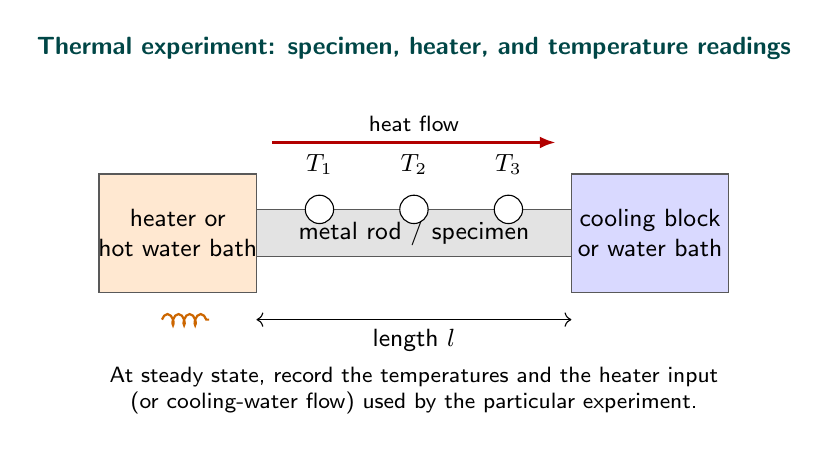
\begin{tikzpicture}[font=\sffamily\small]
\node[font=\sffamily\bfseries\small,text=teal!55!black] at (0,4.1) {Thermal experiment: specimen, heater, and temperature readings};
\draw[fill=orange!18,draw=black!65] (-4,1.0) rectangle (-2.0,2.5);
\node[align=center] at (-3,1.75) {heater or\\hot water bath};
\draw[fill=gray!22,draw=black!65] (-2.0,1.45) rectangle (2.0,2.05);
\node at (0,1.75) {metal rod / specimen};
\draw[fill=blue!15,draw=black!65] (2.0,1.0) rectangle (4,2.5);
\node[align=center] at (3,1.75) {cooling block\\or water bath};
\foreach \x/\lab in {-1.2/$T_1$,0/$T_2$,1.2/$T_3$} {\draw[fill=white] (\x,2.05) circle (.18); \node[above=.12cm] at (\x,2.25) {\lab};}
\draw[-{Latex[length=2mm]},red!70!black,line width=1pt] (-1.8,2.9) -- (1.8,2.9) node[midway,above,black,font=\sffamily\footnotesize]{heat flow};
\draw[decorate,decoration={coil,segment length=4pt,amplitude=2pt},orange!80!black,line width=.8pt] (-3.2,.65) -- (-2.6,.65);
\draw[<->] (-2,0.65) -- (2,0.65) node[midway,below] {length $l$};
\node[align=center,font=\sffamily\footnotesize] at (0,-.25) {At steady state, record the temperatures and the heater input\\(or cooling-water flow) used by the particular experiment.};
\end{tikzpicture}
\end{document}
